\chapter{Märkte und Marktinterventionen}

\section{Märkte}

\begin{definition}
	Gegeben seien eine Nachfragefunktion $D(p)$ und eine Angebotsfunktion $S(p)$ für ein Gut auf einem isolierten Markt.
	Ein partielles Marktgleichgewicht ist ein Preis-Mengen-Paar $(p^*,q^*)$, so dass gilt:
	\[
		D(p^*) = S(p^*) = q^*
		.\]
\end{definition}

Betrachten wir die Stabilitätsbedingung, das heißt, wenn gilt
\[
	\frac{\mathrm{d}}{\mathrm{d}p} \left( S(p) -D(p) \right) \mid_{p=p^*} > 0
	.\]
Dies führt dazu, dass ein Preisanstieg oberhalb $p^*$ zu einem Angebotsüberschuss führt.
Analog geht mit einem Preisrückgang ein Nachfrageüberschuss einher.


\begin{figure}[h]
	\caption{partielles Marktgleichgewicht, mit linearen Nachfrage- und Angebotskurve}
	\begin{center}
		\begin{tikzpicture}[scale=1.2]
			% Achsen
			\draw[->] (0,0) -- (6,0) node[right] {Menge $q$};
			\draw[->] (0,0) -- (0,5) node[above] {Preis $p$};

			% Nachfragefunktion D(p)
			\draw[thick,blue] (0.5,4.5) -- (5.5,0.5) node[below right] {$D(p)$};

			% Angebotsfunktion S(p)
			\draw[thick,red] (0.5,0.5) -- (5.5,4.5) node[above right] {$S(p)$};

			% Gleichgewichtspunkt
			\draw[dashed] (3,0) -- (3,2.5);
			\draw[dashed] (0,2.5) -- (3,2.5);
			\filldraw[black] (3,2.5) circle (2pt) node[above right] {$(q^*, p^*)$};

			% Achsenbeschriftungen
			\node at (3,-0.3) {$q^*$};
			\node at (-0.3,2.5) {$p^*$};

		\end{tikzpicture}

	\end{center}
\end{figure}

Das partielle Marktgleichgewicht kann benutzt werden um zu analysieren was passiert, wenn sich Angebot oder Nachfrage verändern.
Eine solche Analyse als komperative Statik bezeichnet.

\begin{figure}
	\begin{center}
		\caption{Nachfrage und Angebotsveränderung}
		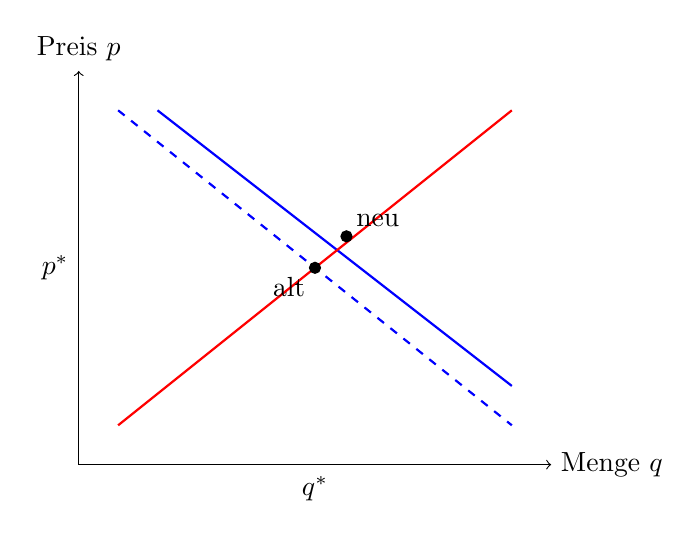
\begin{tikzpicture}[scale=1]
			% Achsen
			\draw[->] (0,0) -- (6,0) node[right] {Menge $q$};
			\draw[->] (0,0) -- (0,5) node[above] {Preis $p$};

			% Alte Nachfrage
			\draw[thick,blue,dashed] (0.5,4.5) -- (5.5,0.5);

			% Neue Nachfrage
			\draw[thick,blue] (1,4.5) -- (5.5,1);

			% Angebot
			\draw[thick,red] (0.5,0.5) -- (5.5,4.5);

			% Gleichgewichtspunkte
			\filldraw[black] (3,2.5) circle (2pt) node[below left] {alt};
			\filldraw[black] (3.4,2.9) circle (2pt) node[above right] {neu};

			% Achsenbeschriftungen
			\node at (3,-0.3) {$q^*$};
			\node at (-0.3,2.5) {$p^*$};

		\end{tikzpicture}



		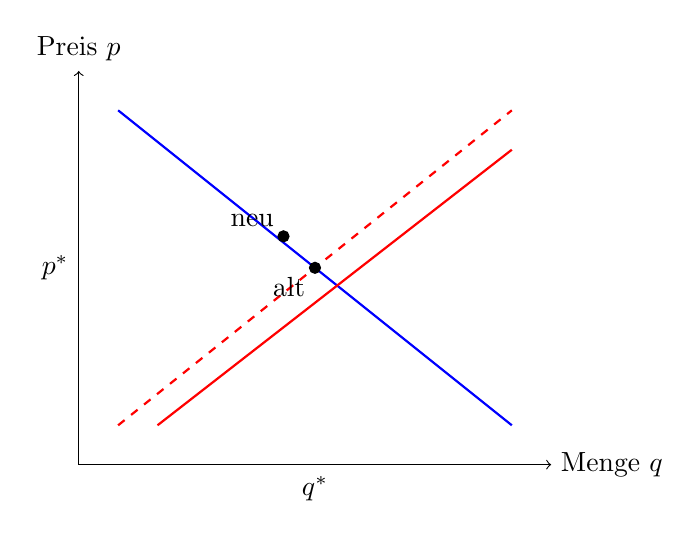
\begin{tikzpicture}[scale=1]
			% Achsen
			\draw[->] (0,0) -- (6,0) node[right] {Menge $q$};
			\draw[->] (0,0) -- (0,5) node[above] {Preis $p$};

			% Nachfrage
			\draw[thick,blue] (0.5,4.5) -- (5.5,0.5);

			% Altes Angebot
			\draw[thick,red,dashed] (0.5,0.5) -- (5.5,4.5);

			% Neues Angebot (linksverschoben)
			\draw[thick,red] (1,0.5) -- (5.5,4);

			% Gleichgewichtspunkte
			\filldraw[black] (3,2.5) circle (2pt) node[below left] {alt};
			\filldraw[black] (2.6,2.9) circle (2pt) node[above left] {neu};

			% Achsenbeschriftungen
			\node at (3,-0.3) {$q^*$};
			\node at (-0.3,2.5) {$p^*$};

		\end{tikzpicture}

	\end{center}

\end{figure}


\begin{remark}
    In dem wir $D(p)$ und $S(p)$ betrachten, nehmen wir implizit an, dass Konsumenten und Produzenten \emph{Preisnehmer} sind, also Preise nicht beeinflussen können.  
\end{remark}


\section{Marktinterventionen}



In unserem bisherigem vorgehen, haben wir staatliche Eingriffe oder andere Friktionen vernachlässigt.
Typischerweise existieren diese, oft sind diese Eingriffe Steuern.

\subsection{Steuern}

Zahlen Produzenten die Steuern, dann verändert sich die Nachfragekurve der Konsumenten nicht, jedoch verändert sich die Angebotskurve bei einer Steuer $t$ gerade:
\[
S'(p) = S(p-t)
,\]
damit verschiebt sich diese genau um $t$ nach oben. 
Zahlen nun Konsumenten die Steuer ergibt sich analog:
\[
D'(p) = D(p+t)
,\]
damit verschiebt nicht die Nachfragekurve genau um $t$ nach unten.

Es entseht unabhängig davon, wer besteuert wird das gleiche Gleichgewicht, wenn die Steuer gleich ist. Jedoch entsteht je nach Besteuerung ein Wohlfahrtsverlust, für entweder Konsument oder Produzent, denn ein Teil der Einnahmen wird nun an den Staat abgegeben.
\begin{definition}
    Die \defemph{Gesamtwohlfahrt} ergibt sich aus der Summe von Konsumenten-, Produzentenrente und staatliche Einnahmen:
    \[
        \operatorname{TW} = \operatorname{CS} + \operatorname{PS} + \operatorname{GR}
    .\] 
    Der Wohlfahrtsverlust ergibt sich aus dem Wert, den die Gesamtwohlfahrt nach der Steuer sinkt. 
\end{definition}

\subsection{Preisgrenzen}





\subsection{Zölle und Quoten}

Damit wir Zöllen und Quoten überhaupt behandeln können, müssen wir handel zu lassen.


\begin{definition} \index{Freihandel}
	Eine Situation, in der uneingeschränkt gehandelt werden kann, wird als
	\defemph{Freihandel} bezeichnet.
\end{definition}

Handel ergibt nur Sinn, wenn der internationale Angebotspreis unterhalb des lokalen Angebotspreis ist.


Neben Zoll auf die Güter, kann es auch Quoten geben, die den Import auf gewisse Güter auf eine Menge beschränkt wird.



\section{Allgemeines Gleichgewicht}
Im partiellen Gleichgewichtsmodell haben wir nur ein einziges Gut
angeschaut und gefragt für welchen Preis \enquote{Angebot gleich Nachfrage} gilt.

Allgemein versuchen wir, die Variablen, die im partiellen Gleichgewichtsmodell exogen gegeben sind,
zu endogenisieren.


\subsection{Robinson-Cruse-Modell}


\subsection{Walras'sche Gesetz}




\subsection{Pareto-Effizenz}


\begin{theorem}[1. Wohlfahrtstheorem]
	Die Allokation in unserer Ökonomie mit zwei
	Gütern und zwei Konsumenten ist Pareto effizient wenn die Konsumenten
	monotone Präferenzen haben
\end{theorem}

\begin{proof}
	tbd
\end{proof}

\begin{remark}
	Arbeitsmärkte und Bevölkerungsökonomik
\end{remark}


\section{Kapitaleinkommen Besteuerung}
Einkommen aus Kapital fließt vor allem reichen Leuten zu. Viele Leute
empfinden deshalb eine Kapitalsteuer, die mindestens so hoch ist wie eine
Lohnsteuer, als gerecht. Parteien wie z.B. die FDP argumentieren dagegen
manchmal, dass eine geringe Kapitalsteuer allen Gesellschaftsschichten zu
Gute kommt, da ein günstiges Investitionsklima den Arbeitsmarkt
stimuliert, Gehälter erhöht und Arbeitslosigkeit senkt.
Ist es der Fall, dass eine geringere Kapitalsteuer zu höheren Gehältern für
Arbeiter führt?

\begin{remark}
	Ein weiteres Argument gegen hohe Steuern auf Kapital ist
	Steuerflucht, getreu dem Motto \enquote{Besser $25$ Prozent von X als $45$ Prozent
		von nix.}
\end{remark}


Da es aber offensichtlich ist, warum Steuerflucht als ein Argument gegen
hohe Steuern auf Kapital bzw. Kapitalerträge benutzt werden kann (und
nur die Größe des Effekts umstritten ist) werden wir uns mit der Frage
beschäftigen ob Steuern auf Kapital zu höheren Gehältern führen oder
nicht, die viel umstrittener und daher interessanter ist.


\begin{remark}
	Ist die Rendite bei Kapitalanlagen fix macht es keinen
	großen Unterschied ob Sie Kapitalerträge oder Kapitalanlagen besteuern.
\end{remark}
\begin{example}
	Nehmen wir z.B. eine Steuer auf Kapitalerträge von $25\%$. Ist die Rendite
	$10\%$ so bedeutet dies, dass von einer Kapitalanlage von $X$ Euro eine Steuer
	in der Höhe von $25\%\cdot (10\%\cdot X)$ gezahlt wird. Da $25\%\cdot (10\%\cdot X) = 2,5\%\cdot X$
	ist dies das Gleiche wie eine Steuer auf Kapitalanlagen von $2,5\%$.
	Nehmen wir einfachheitshalber an, dass Renditen für verschiedene Einlagen
	in etwa gleich sind, so macht es daher keinen Unterschied ob wir eine
	Erhöhung einer Steuer auf Kapitalanlagen oder die Erhöhung einer Steuer
	auf Kapitalerträge betrachten.
\end{example}
